A complete example of how to run the \glsentryfull{qmla} framework, 
    including how to implement a custom \glsentryfull{es}, 
    and generate/interpret analysis, is given.
\par 

First, \emph{fork} the \gls{qmla} codebase from \cite{flynn2021QMLA}\footnotemark.
\footnotetext{This will require a Github account.} 
Now, we must download the code base and ensure it runs properly;
    these instructions are implemented via the command line\footnotemark. 
\footnotetext{
    Note: these instructions are tested for Linux and presumed to work on Mac, but untested on Windows. 
    It is likely some of the underlying software (redis servers) can not be installed on Windows. 
}
    
\begin{lstlisting}[
    label=listing:qmla_setup,
    caption={QMLA codebase setup},
    language=Bash
]
# Install redis (database broker)
sudo apt update
sudo apt install redis-server
 
# make directory for QMLA
cd
mkdir qmla_test
cd qmla_test

# make Python virtual environment for QMLA
# note: change Python3.6 to desired version
sudo apt-get install python3.6-venv 
python3.6 -m venv qmla-env    
source qmla-env/bin/activate

# Download QMLA
git clone --depth 1 https://github.com/username/QMLA.git # REPLACE username

# Install dependencies
cd QMLA 
pip install -r requirements.txt  # note there may be a problem with matplotlib version; just pip install it directly
\end{lstlisting}

When all of the requirements are installed, test the framework runs. 
\gls{qmla} uses \ttt{redis} databases to store intermittent data:
    we must manually initialise the database. 
Run the following 
    (note: here we list \ttt{redis-4.0.8}, but this must be corrected to reflect the 
    version installed on the user's machine in the above setup section):
\begin{lstlisting}[
    label=listing:athlete_class,
    caption={Launch redis database},
    language=Bash
]
~/redis-4.0.8/src/redis-server
\end{lstlisting}

which should give something like \cref{fig:terminal_redis}.
\begin{figure}
    \begin{center}
        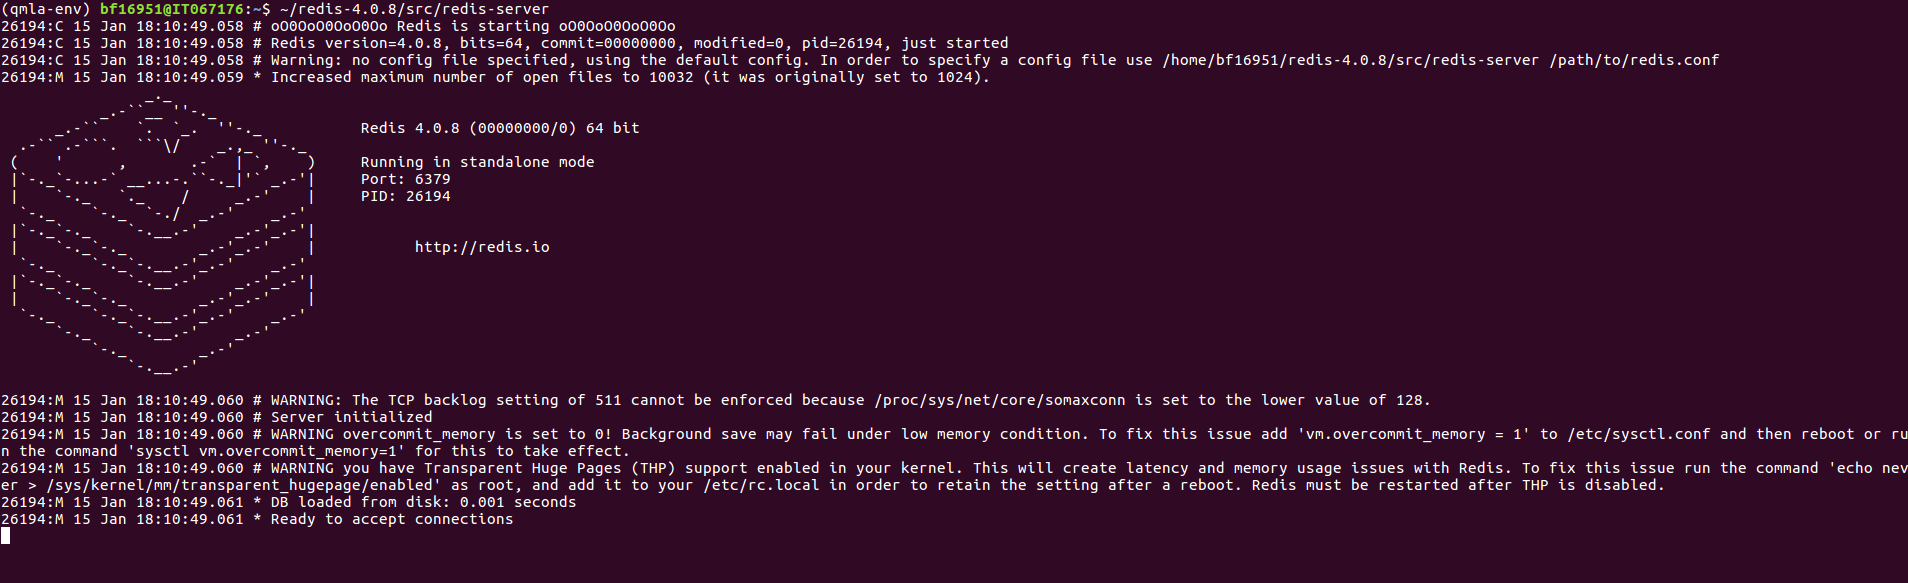
\includegraphics[width=0.9\textwidth]{appendix/figures/terminal_redis.png}
    \end{center}
    \label{fig:terminal_redis}
    \caption[Terminal running redis-server]{Terminal running \ttt{redis-server}.}
\end{figure}
\par 

In a text editor, open \ttt{qmla\_test/QMLA/launch/local\_launch.sh}; 
    here we will ensure that we are running the \gls{qhl} algorithm, 
    with 5 experiments and 20 particles, on the \gls{es} named \ttt{ExampleBasic}.
Ensure the first few lines of \ttt{local\_launch.sh} read:

\begin{lstlisting}[
    label=listing:local_launch,
    caption={\ttt{local\_launch} script},
    language=Bash
]
    
#!/bin/bash

###############
# QMLA run configuration
###############
num_instances=1
run_qhl=1 # perform QHL on known (true) model
run_qhl_multi_model=0 # perform QHL for defined list of models.
exp=5 # number of experiments
prt=20 # number of particles

###############
# QMLA settings - user
###############
plot_level=5
debug_mode=0

###############
# QMLA settings - default
###############
do_further_qhl=0 # QHL refinement to best performing models 
q_id=0 # isntance ID can start from other ID if desired
use_rq=0
further_qhl_factor=1
further_qhl_num_runs=$num_instances
plots=0
number_best_models_further_qhl=5

###############
# Choose an exploration strategy 
# This will determine how QMLA proceeds. 
###############

exploration_strategy="ExampleBasic"
\end{lstlisting}    

Now we can run 
Ensure the terminal running redis is kept active, and open a separate terminal window. 
We must activate the Python virtual environment configured for \gls{qmla}, 
which we set up in \cref{listing:qmla_setup}. 
Then, we navigate to the \gls{qmla} directory, and launch:
\begin{lstlisting}[
    label=listing:launch_example,
    caption={Launch QMLA},
    language=Bash
]

# activate the QMLA Python virtual environment 
source qmla_test/qmla-env/bin/activate

# move to the QMLA directory 
cd qmla_test/QMLA
# Run QMLA
cd launch   
./local_launch.sh

\end{lstlisting}

There may be numerous warnings, but they should not affect whether \gls{qmla} has succeeded; 
    \gls{qmla} will \ttt{raise} any significant error. 
Assuming the run has completed successfully, \gls{qmla} stores the run's results in a subdirectory
    named by the date and time it was started.  
Plots/analysis are generated at the \gls{instance} and \gls{model} level;
    each results directory has an \ttt{analyse.sh} script to generate plots at the \gls{run} level. 
For examples, if the run was initialised on January $1^{st}$ at 01:23 navigate to that directory and analyse it by

\begin{lstlisting}[
    label=listing:results_directory,
    caption={QMLA results directory},
    language=Bash
]
cd results/Jan_01/01_23
./analyse.sh
\end{lstlisting}

For now it is sufficient to notice that the code has sun successfully and the analysis has generated several new files and directores; 
    in the following sections we will describe the outputs. 

\section{Custom \glsentrylong{es}}

Next, we design a basic \gls{es}, for the purpose of demonstrating how to run the algorithm.
\glspl{es} are placed in the directory \ttt{qmla/exploration\_strategies}. 
To make a new one, navigate to the exploration strategies directory, 
make a new subdirectory, and copy the template file. 

\begin{lstlisting}[
    label=listing:athlete_class,
    caption={QMLA codebase setup},
    language=Bash
]

cd ~/qmla_test/QMLA/exploration_strategies/
mkdir custom_es

# Copy template file into example
cp template.py custom_es/example.py
cd custom_es

\end{lstlisting}

Ensure \gls{qmla} will know where to find the \gls{es} by importing everything from the custom \gls{es} 
    directory into to the main \ttt{exploration\_strategy} module. 
Then, in the \ttt{custom\_es} directory, make a file called \ttt{\_\_init\_\_.py} which imports the new \gls{es}
    from the \ttt{example.py} file. 
To add any further \glspl{es} inside the directory \ttt{custom\_es}, include them in the custom \ttt{\_\_init\_\_.py},
    and they will automatically be available to \gls{qmla}.

\begin{lstlisting}[
    label=listing:athlete_class,
    caption={QMLA codebase setup},
    language=Python
]

# inside qmla/exploration_strategies/custom_es
#  __init__.py    
from qmla.exploration_strategies.custom_es.example import *

# inside qmla/exploration_strategies, add to the existing
# __init__.py 
from qmla.exploration_strategies.custom_es import *

\end{lstlisting}

Now, change the structure (and name) of the \gls{es} inside \ttt{custom\_es/example.py}. 
Say we wish to target the true model 
\begin{equation}
    \label{eqn:example_es_true_ham}
    \begin{split}
        \al &= \irow{ \alpha_{1,2} & \alpha_{2,3} & \alpha_{3,4}} \\
        \terms &= \icol{ \sz^1 \otimes \sz^2 \\ \sz^2 \otimes \sz^3  \\ \sz^3 \otimes \sz^4 } \\
        \Longrightarrow \ho &= \sz^{(1,2)} \sz^{(2,3)} \sz^{(3,4)} \\
    \end{split}
\end{equation}

\gls{qmla} interprets models as strings, where terms are separated by \ttt{+}, and parameters are implicit. 
So the target model in \cref{eqn:example_es_true_ham} will be given by 
$$ \ttt{pauliSet\_1J2\_zJz\_d4+pauliSet\_2J3\_zJz\_d4+pauliSet\_3J4\_zJz\_d4}. $$

Adapting the template \gls{es} slightly, we can define a model generation strategy with a small number of hard coded 
    candidate models introduced at the first and second branch of the \glsentrylong{et}. 
We will also set the parameters of the terms which are present in $\ho$, as well as the range in which to search parameters.
Keeping the \ttt{import}s at the top of the \ttt{example.py}, rewrite the \gls{es} as: 

\begin{lstlisting}[
    label=listing:athlete_class,
    caption={QMLA codebase setup},
    language=Python
]
class ExampleBasic(
    exploration_strategy.ExplorationStrategy
):

    def __init__(
        self,
        exploration_rules,
        true_model=None,
        **kwargs
    ):
        self.true_model = 'pauliSet_1J2_zJz_d4+pauliSet_2J3_zJz_d4+pauliSet_3J4_zJz_d4'
        super().__init__(
            exploration_rules=exploration_rules,
            true_model=self.true_model,
            **kwargs
        )

        self.initial_models = None
        self.max_spawn_depth = 1
        self.true_model_terms_params = {
            'pauliSet_1J2_zJz_d3' : 2.5,
            'pauliSet_2J3_zJz_d3' : 7.5,
            'pauliSet_4J5_zJz_d3' : 3.5,
        }
        self.min_param = 0
        self.max_param = 10

    def generate_models(self, **kwargs):

        self.log_print(["Generating models; spawn step {}".format(self.spawn_step)])
        if self.spawn_step == 0:
            # chains up to 4 sites
            new_models = [
                'pauliSet_1J2_zJz_d4',
                'pauliSet_1J2_zJz_d4+pauliSet_2J3_zJz_d4',
                'pauliSet_1J2_zJz_d4+pauliSet_2J3_zJz_d4+pauliSet_3J4_zJz_d4',
            ]
            
        elif self.spawn_step == 1:
            new_models = [
                'pauliSet_1J2_zJz_d4+pauliSet_1J4_zJz_d4+pauliSet_2J3_zJz_d4+pauliSet_3J4_zJz_d4', # ring
                'pauliSet_1J2_zJz_d4+pauliSet_1J3_zJz_d4+pauliSet_2J4_zJz_d4+pauliSet_3J4_zJz_d4', # square
            ]

        return new_models

\end{lstlisting}


To run\footnotemark \ the example \gls{es}, return to the \ttt{local\_launch} of \cref{listing:local_launch}, 
    but change some of the settings:
\begin{lstlisting}[
    label=listing:example_es_qhl_run,
    caption={\ttt{local\_launch} configuration for QHL},
    language=Bash
]
prt=2000
exp=500
run_qhl=1
exploration_strategy=ExampleBasic
\end{lstlisting}

Run locally again as in \cref{listing:launch_example}, move to the results directory and analyse its contents as in \cref{listing:results_directory}. 
\footnotetext{Note this will take up to 20 minutes to run.}
\par 
\gls{qmla} stores results, and generates plots, 
    over the entire range of the algorithm, i.e. the \gls{run}\footnotemark, \gls{instance} and models. 
\footnotetext{Recall that a single implementation of \gls{qmla} is called an \gls{instance},    
    and a series of instances which share the same target model is called the \gls{run}.}
The depth of analysis performed automatically is the user control \ttt{plot\_level} in \ttt{local\_launch.sh};
    for \ttt{\plot\_level=1}, only the most basic figures are generated, while \ttt{\plot\_level=6} generates plots for every individual 
    model considered. 
For model searches across large model spaces and/or considering many candidates,
    excessive plotting can cause considerable slow-down, so users should be careful to generate plots only 
    to the degree they will be useful. 
\par 

We have just run \glsentryfull{qhl} for the model in \cref{eqn:example_es_true_ham} for a single instance, 
    using a reasonable number of particles and experiments, so we expect to have trained the model well. 
Instance-level results are stored (e.g. for the instance with \ttt{qmla\_id=1}) in \ttt{Jan\_01/01\_23/instances/qmla\_1}.
Individual models' insights can be found in \ttt{model\_training}, 
    e.g. the training is summarised as in \cref{fig:qmla_learning_summary}, with the resultant dynamics in \cref{fig:qmla_model_dynamics}.
\par 
\begin{figure}
    \begin{center}
        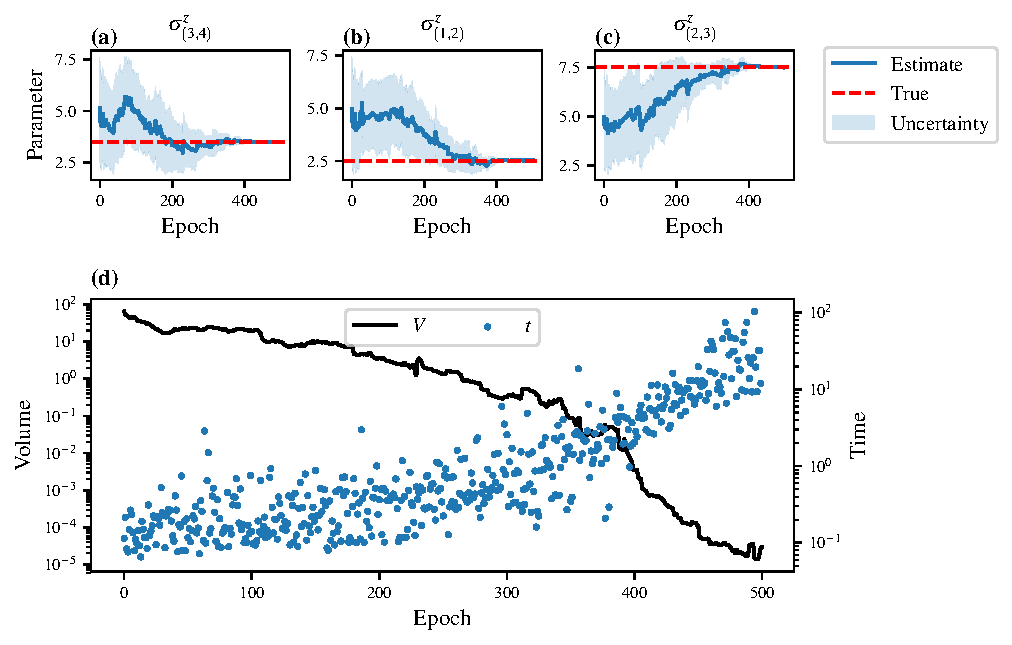
\includegraphics{qmla_run_data/Jan_15/23_23/single_instance_plots/qmla_2/model_training/learning_summary_1.png}
    \end{center}
    \caption[ \gls{qmla} plot: learning\_summary]{
        \gls{qmla} plot: \ttt{model\_trainings/learning\_summary}. 
        Displays the outcome of \gls{qhl} for the given model:
        \textbf{(a)}-\textbf{c} show the estaimates of the parameters; 
        \textbf{(d)} shows the total parameterisation volume against experiments trained upon, 
        along with the evolution times used for those experiments. 
    }
    \label{fig:qmla_learning_summary}
\end{figure}
\begin{figure}
    \begin{center}
        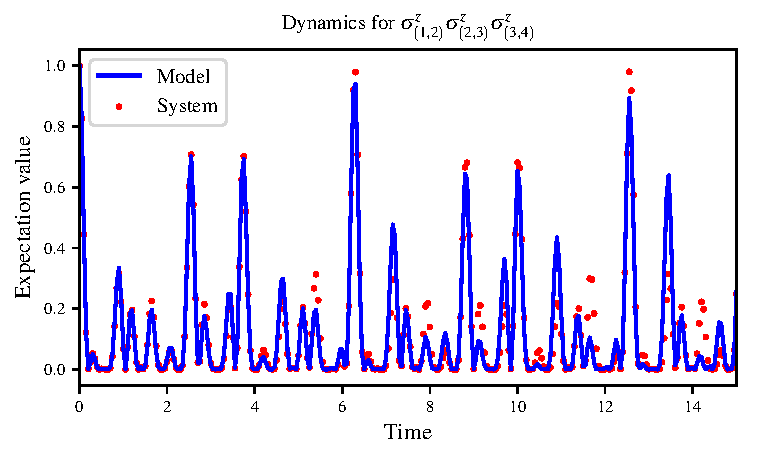
\includegraphics{qmla_run_data/Jan_15/23_23/single_instance_plots/qmla_2/model_training/dynamics_1.pdf}
    \end{center}
    \caption[ \gls{qmla} plot: dynamics]{
        \gls{qmla} plot: \ttt{model\_trainings/dynamics}. 
        Displays the outcome of \gls{qhl} for the given model:
        its attempt at reproducing data from $\ho$. 
    }
    \label{fig:qmla_model_dynamics}
\end{figure}

In this case, because we are running \gls{qhl}, there is little analysis of interest besides the single model's training, 
    as shown already. 
It is of interest, however, to consider analysis on the \gls{run} level, i.e. the average result of the training 
    of the true model over several instances. 
This can be achieved by settig \ttt{num\_instances} in \ttt{local\_launch.sh}. 
For example, set \ttt{num\_instances=10}, \ttt{prt=50}, \ttt{exp=10}, then launch and analyse the results (\cref{listing:results_directory}). 
In this case, since we are using few resources, the training will be ineffective, 
    but ensure run-level analyses are generated in the results directory, e.g. in subdirectories \ttt{performance} and \ttt{champion\_models}. 
\par 



